\documentclass[12pt]{article}
\usepackage{geometry}
\geometry{a4paper, margin=1in}
\usepackage{setspace}
\usepackage{graphicx}
\usepackage{titlesec}
\usepackage{enumitem}
\usepackage{tikz}
\usetikzlibrary{arrows.meta, positioning, backgrounds, fit}
\usepackage{mathptmx} % Times font

\titleformat{\section}{\normalfont\Large\bfseries}{\thesection}{1em}{}
\titleformat{\subsection}{\normalfont\large\bfseries}{\thesubsection}{1em}{}

\begin{document}
\begin{center}
    \LARGE \textbf{EduChat: AI-Powered Educational Assistant}\\[1em]
    \large Final Project Report\\[2em]
\end{center}

\section{Introduction}
EduChat is an AI-powered educational assistant designed to revolutionize the way students interact with their study materials. Leveraging advanced natural language processing and retrieval-augmented generation (RAG) technologies, EduChat provides personalized, context-aware responses to academic questions. Unlike generic AI chatbots, EduChat processes and understands students' actual educational documents, such as textbooks and lecture notes, enabling highly specific and relevant answers based on their own study materials. The system combines local language model processing with a sophisticated document understanding pipeline, allowing students to upload PDFs and receive instant, accurate responses to queries about complex academic concepts. EduChat serves as a 24/7 learning companion, enhancing comprehension, retention, and academic performance.

\section{Problem Statement}
Modern education presents several significant challenges that EduChat aims to address:
\begin{itemize}[leftmargin=2em]
    \item \textbf{Information Overload:} Students are often overwhelmed by extensive textbooks, lecture notes, and reference materials. Finding specific information quickly becomes difficult, leading to inefficient study sessions and frustration.
    \item \textbf{Limited Access to Personalized Help:} Many students lack access to immediate, personalized academic assistance outside of class hours. When struggling with concepts late at night before an exam, help might not be available.
    \item \textbf{Contextual Understanding Gaps:} Generic search engines and AI tools provide general information but fail to connect it to a student's specific curriculum or learning materials.
    \item \textbf{Digital Divide in Educational Support:} Advanced educational support tools are often expensive, internet-dependent, or require high-end hardware, creating accessibility barriers.
    \item \textbf{Privacy and Data Security Concerns:} Many online educational tools collect extensive student data and require internet connectivity, raising privacy concerns for educational institutions and parents.
\end{itemize}
EduChat addresses these challenges by providing an offline, privacy-focused solution that processes students' actual study materials to deliver contextually relevant answers. By running locally on standard consumer hardware and working directly with students' documents, it bridges the gap between generic AI assistants and the specific needs of educational contexts.

\section{Project Description}
EduChat is a comprehensive educational assistant system that uses local language model processing and document understanding to help students learn from their study materials. The project consists of several integrated components:

\subsection{User Interface and Experience}
EduChat features a clean, intuitive web-based interface built with Flask, Bootstrap, and JavaScript. Users can register accounts, upload documents, and engage in natural conversations with the AI assistant. The interface is designed to be familiar to students who use modern chat applications, with a document sidebar for managing study materials and a conversation area for interacting with the AI.

Key UI features include:
\begin{itemize}[leftmargin=2em]
    \item Document upload and management system
    \item Real-time chat interface with typing indicators
    \item Document selection for context-specific queries
    \item Chat history with persistent conversations
    \item Mobile-responsive design for use across devices
\end{itemize}

\subsection{Document Processing Pipeline}
The system employs a sophisticated document processing pipeline that transforms raw PDFs into queryable knowledge:
\begin{itemize}[leftmargin=2em]
    \item \textbf{PDF Extraction:} Using PyMuPDF (fitz), the system extracts text while preserving structure and handling multi-column layouts common in academic texts.
    \item \textbf{Text Cleaning:} Removes headers, footers, and other non-content elements that could confuse the AI.
    \item \textbf{Semantic Chunking:} Rather than arbitrary text splitting, the system uses sentence embeddings to create coherent chunks based on semantic similarity.
    \item \textbf{Vector Embedding:} Each chunk is converted to a high-dimensional vector representation using a sentence transformer model.
    \item \textbf{Vector Database Storage:} Embeddings are indexed using FAISS for efficient similarity search.
\end{itemize}

\subsection{Retrieval-Augmented Generation (RAG) System}
The heart of EduChat is its RAG system, which combines document retrieval with language model generation:
\begin{itemize}[leftmargin=2em]
    \item \textbf{Query Understanding:} Student questions are converted to vector embeddings.
    \item \textbf{Semantic Search:} The system retrieves the most relevant chunks from the document based on semantic similarity.
    \item \textbf{Context Assembly:} Retrieved chunks are assembled with the query into a prompt.
    \item \textbf{Response Generation:} A locally-running language model (Llama 3.1 8B Instruct) generates responses based on the document context.
    \item \textbf{Response Cleaning:} Post-processing improves readability by removing artifacts and formatting the response.
\end{itemize}

\subsection{Conversation Memory}
To provide a more natural interaction experience, EduChat includes:
\begin{itemize}[leftmargin=2em]
    \item Per-session conversation tracking
    \item Context-aware responses that reference previous exchanges
    \item Automatic memory management to handle long conversations
    \item Session persistence across page refreshes
\end{itemize}

\subsection{Database and Storage}
The system uses:
\begin{itemize}[leftmargin=2em]
    \item SQLite database for user accounts, document metadata, and chat history
    \item FAISS vector database for document embeddings
    \item File system storage for uploaded documents
\end{itemize}

\subsection{Offline Processing Capability}
A key feature of EduChat is its ability to run entirely locally:
\begin{itemize}[leftmargin=2em]
    \item CPU-optimized language model inference
    \item No data sent to external servers
    \item Full functionality without internet connection
\end{itemize}

\section{Project Flowchart}
Below is a flowchart illustrating the transition between each component of the EduChat project:

\begin{figure}[h!]
\centering
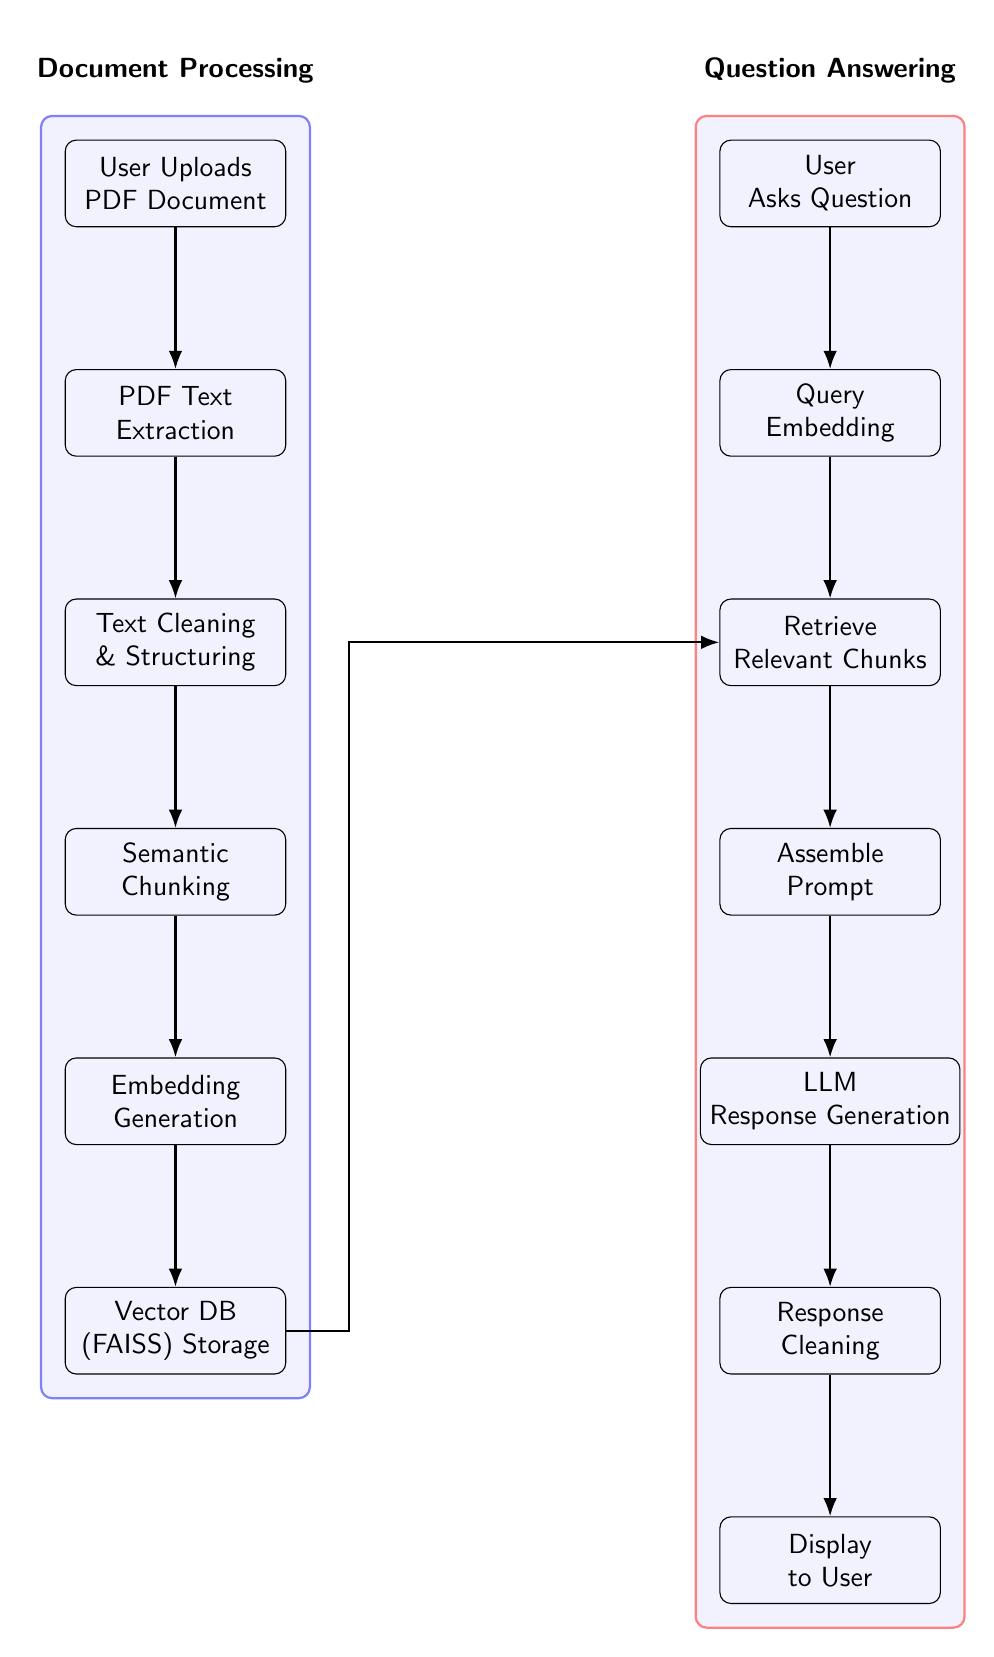
\begin{tikzpicture}[
    node distance=1.8cm and 2.5cm,
    every node/.style={font=\sffamily, align=center, minimum width=2.8cm, minimum height=1.1cm, draw, rounded corners, fill=blue!5},
    arrow/.style={-Latex, thick}
]

% Nodes
\node (upload) {User Uploads\\PDF Document};
\node (extract) [below=of upload] {PDF Text\\Extraction};
\node (clean) [below=of extract] {Text Cleaning\\\& Structuring};
\node (chunk) [below=of clean] {Semantic\\Chunking};
\node (embed) [below=of chunk] {Embedding\\Generation};
\node (vector) [below=of embed] {Vector DB\\(FAISS) Storage};

\node (chat) [right=5.5cm of upload] {User\\Asks Question};
\node (qembed) [below=of chat] {Query\\Embedding};
\node (retrieve) [below=of qembed] {Retrieve\\Relevant Chunks};
\node (prompt) [below=of retrieve] {Assemble\\Prompt};
\node (llm) [below=of prompt] {LLM\\Response Generation};
\node (cleanresp) [below=of llm] {Response\\Cleaning};
\node (display) [below=of cleanresp] {Display\\to User};

% Arrows for document processing
\draw[arrow] (upload) -- (extract);
\draw[arrow] (extract) -- (clean);
\draw[arrow] (clean) -- (chunk);
\draw[arrow] (chunk) -- (embed);
\draw[arrow] (embed) -- (vector);

% Arrows for question answering
\draw[arrow] (chat) -- (qembed);
\draw[arrow] (qembed) -- (retrieve);
\draw[arrow] (retrieve) -- (prompt);
\draw[arrow] (prompt) -- (llm);
\draw[arrow] (llm) -- (cleanresp);
\draw[arrow] (cleanresp) -- (display);

% Cross arrows for context retrieval
\draw[arrow] (vector.east) -- ++(0.8,0) |- (retrieve.west);

% Dashed box for Document Processing
\begin{scope}[on background layer]
\node[draw=blue!50, thick, rounded corners, fit=(upload) (vector), inner sep=0.3cm, label=above:{\textbf{Document Processing}}] {};
\end{scope}

% Dashed box for Question Answering
\begin{scope}[on background layer]
\node[draw=red!50, thick, rounded corners, fit=(chat) (display), inner sep=0.3cm, label=above:{\textbf{Question Answering}}] {};
\end{scope}

\end{tikzpicture}
\caption{EduChat System Flowchart: Document Processing and Question Answering}
\end{figure}

\section{Technologies Used}
EduChat integrates various technologies across its stack:

\textbf{Frontend:}
\begin{itemize}[leftmargin=2em]
    \item HTML/CSS/JavaScript for the user interface
    \item Bootstrap 5 for responsive design components
    \item jQuery for DOM manipulation and AJAX requests
    \item Font Awesome for iconography
\end{itemize}

\textbf{Backend:}
\begin{itemize}[leftmargin=2em]
    \item Flask web framework for server-side processing
    \item Flask-Login for user authentication
    \item SQLAlchemy for database ORM
    \item Werkzeug for security and file handling
\end{itemize}

\textbf{Natural Language Processing:}
\begin{itemize}[leftmargin=2em]
    \item Llama 3.1 8B Instruct (quantized) for text generation
    \item Sentence-Transformers for semantic embeddings
    \item NLTK for text tokenization and processing
    \item llama-cpp-python for optimized CPU inference
\end{itemize}

\textbf{Document Processing:}
\begin{itemize}[leftmargin=2em]
    \item PyMuPDF (fitz) for PDF text extraction
    \item Custom semantic chunking algorithm
    \item FAISS for vector indexing and similarity search
\end{itemize}

\textbf{Data Storage:}
\begin{itemize}[leftmargin=2em]
    \item SQLite for relational database needs
    \item FAISS for vector database functionality
    \item File system for document storage
\end{itemize}

\textbf{Optimization:}
\begin{itemize}[leftmargin=2em]
    \item PyTorch quantization for model efficiency
    \item Batch processing for embedding generation
    \item CPU threading optimization for better performance
\end{itemize}

\section{Cost Analysis}
Implementing EduChat in a real-world context in Bangladesh is highly cost-effective due to the use of open-source software and local hardware. The main costs are:

\begin{itemize}[leftmargin=2em]
    \item \textbf{Development:} Minimal, as all core components (Flask, PyTorch, FAISS, NLTK, etc.) are open source and free.
    \item \textbf{Hardware:} A standard desktop or laptop (8GB+ RAM, 4+ core CPU) is sufficient. Approximate cost: 40,000-60,000 BDT (one-time).
    \item \textbf{Internet:} Only needed for initial setup and model download; regular use is offline.
    \item \textbf{Maintenance:} Occasional updates and backups, which can be managed by existing IT staff or a tech-savvy user.
\end{itemize}

There are no recurring license fees, no cloud hosting costs, and no per-user charges. For a school or coaching center, the total cost is limited to the hardware and initial setup, making EduChat a very affordable solution for Bangladesh's education sector.

\section{Conclusion}
EduChat represents a significant advancement in AI-assisted education by providing personalized, context-aware learning support that works directly with students' actual study materials. By combining document understanding, local language model processing, and an intuitive user interface, the system delivers several key benefits:

\textbf{Educational Impact:} EduChat transforms how students interact with their study materials, providing instant clarification on complex concepts and helping them make connections between related topics. This just-in-time assistance can reduce frustration, improve comprehension, and increase study efficiency. The conversational nature of the interface makes advanced AI assistance accessible to students of all technical ability levels.

\textbf{Technical Achievements:} The project successfully demonstrates that sophisticated AI capabilities can be delivered entirely locally on consumer hardware, without requiring expensive cloud services or high-end GPUs. The integration of semantic chunking, vector search, and optimized language model inference creates an effective RAG system that rivals cloud-based alternatives while maintaining privacy and offline accessibility.

\textbf{Accessibility and Inclusion:} By running locally and working with students' actual materials, EduChat addresses several digital divide issues present in education technology. Students without reliable internet access can use the system offline, and the ability to work with any PDF document means it adapts to various curricula, languages, and educational contexts.

\textbf{Future Directions:} EduChat's modular architecture provides a foundation for several promising extensions:
\begin{itemize}[leftmargin=2em]
    \item Multi-modal support for images, diagrams, and mathematical equations
    \item Collaborative features allowing teachers to review student interactions
    \item Integration with learning management systems
    \item Support for additional document formats beyond PDF
    \item Fine-tuning capabilities for specific subjects or educational levels
\end{itemize}

\textbf{Limitations and Challenges:} While EduChat represents a significant step forward, challenges remain in handling complex diagrams, mathematical notation, and ensuring complete factual accuracy. The system's effectiveness is also dependent on the quality of uploaded materials and the underlying language model's capabilities.

In conclusion, EduChat demonstrates the potential for AI to serve as an accessible, personalized educational assistant that respects privacy and works with students' actual learning materials. By bringing advanced language model capabilities to local devices and focusing specifically on educational needs, it offers a meaningful contribution to the future of technology-enhanced learning.

\end{document}